\section{Вариантные расчеты}
Для определения оптимальных степеней повышения давления в компрессорах
построим графики зависимости КПД, удельной мощности и расхода через компрессоры от суммарной степени повышения давления в компрессорах.
При этом для наглядности отнесем абсолютные значения рассматриваемых величин к максимальному значению,
достигающемуся на заданном промежутке.

График зависимостей КПД,
мощности и расхода ГТА от суммарной степени повышения давления в компрессорах представлен на рис. 1. Распределение степеней повышения
давления между компрессорами соответствует оптимальному по КПД:
\begin{figure}[H]
    \centering
	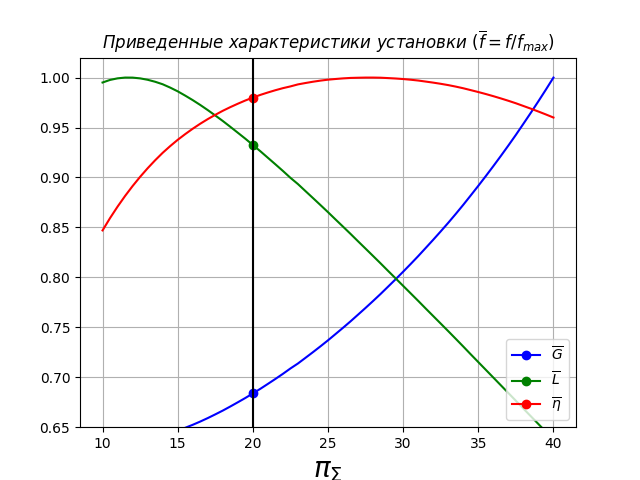
\includegraphics[scale=0.7]{cycle_eta_plot}
	\caption{Характеристики установки}
\end{figure}

Экстремум по КПД достигается при следующих значения функций:
\begin{center}
	\begin{tabular}{|c|c|c|c|c|}
	\hline
		$G, кг/с$ & $N_e, Вт/кг$ & $\eta_e$ & $\pi_{кнд}$ & $\pi_{квд}$ \\ \hline
		$<-<.MaxEta.MassRate | Round1>->$ &
		$<-<.MaxEta.SpecificPower | DivideE6 | Round3>-> \cdot 10^6$ &
		$<-<.MaxEta.Efficiency | Round3>->$ &
		$<-<.MaxEta.PiLow | Round1>->$ &
		$<-<.MaxEta.PiHigh | Round1>->$ \\ \hline
	\end{tabular}
\end{center}

Экстремум по удельной мощности достигается при следующих значениях функций:
\begin{center}
	\begin{tabular}{|c|c|c|c|c|}
	\hline
		$G, кг/с$ & $N_e, Вт/кг$ & $\eta_e$ & $\pi_{кнд}$ & $\pi_{квд}$ \\ \hline
		$<-<.MaxLabour.MassRate | Round1>->$ &
		$<-<.MaxLabour.SpecificPower | DivideE6 | Round3>-> \cdot 10^6$ &
		$<-<.MaxLabour.Efficiency | Round3>->$ &
		$<-<.MaxLabour.PiLow | Round1>->$ &
		$<-<.MaxLabour.PiHigh | Round1>->$ \\ \hline
	\end{tabular}
\end{center}

В связи с высокой температурой за камерой сгорания, для изготовления лопаточных венцов турбины высокого давления требуется
использование крайне дорогих материалов и применение интенсивного охлаждения. Поэтому уменьшение количества ступеней
турбины высокого давления является актуальной технико-экономической задачей. Опираясь на данные вариантного расчета,
можно сказать, что применение в данной схеме двуступенчатой турбины высокого давления приведет к недогрузке
обеих ступеней, а, следовательно, к излишним расходам на материалы. В связи с этим в данной работе принимается
$\pi_{\sum} = <-<.PiTotal | Round1>->$, $\pi_{кнд} = <-<.PiLow | Round1>->$, $\pi_{квд} = <-<.PiHigh | Round1>->$,
что позволит создать эффективную одноступенчатую турбину высокого давления.

Ниже представлен расчет цикла ГТА при $\pi_{кнд} = <-<.PiLow | Round1>->$, $\pi_{квд} = <-<.PiHigh | Round1>->$.
\clearpage